\setchapterpreamble[u]{\margintoc}
\chapter{First Lecture}
\labch{lec1}

% Divide Graphviz Images Width by 95 pixel then round.

\section{Introduction}
\labsec{sec1.1}

\begin{description}
	\item[Analysis of linear continuous system] analysis of a system means simply checking the goodness of its measure of performance.
Analysis could be done in two different ways:
\begin{itemize}
	\item In the lab: by putting test input to the system and checking if the output satisfies the measure of performance.
	\item Using analytical techniques: which is our concern in this course.
\end{itemize}
	\item[The first step] is to make a mathematical model to the system. \\[+1mm]
	$\Sigma F_x = m\ddot{x}$\\
	$F - \mu\dot{x} + kx = m\ddot{x}$\\
	$\therefore$
	\fbox{
	    \parbox{3cm}{
	    $\ F = m\ddot{x} + \mu\dot{x} + kx$
    		}
	}\\[-2mm]
	\item[Then] defining the measure of performance and studying how we can check these measure of performance.
\end{description}

\begin{marginfigure}[-3cm]
		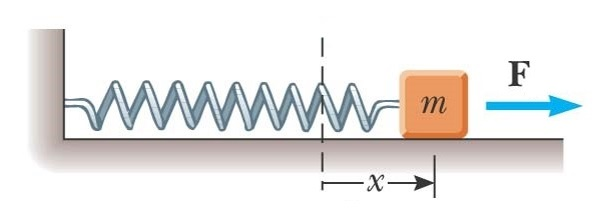
\includegraphics{lec1/Dynamics}
		\caption[Spring problem: figure]{A block attached to a spring.\linkC{https://slideplayer.com/slide/677255/}}
		\labfig{dynamicsSystemFigure}
\end{marginfigure}

 \leavevmode\\[-1.55cm]
 \begin{figure}[hb]
		\raggedleft
		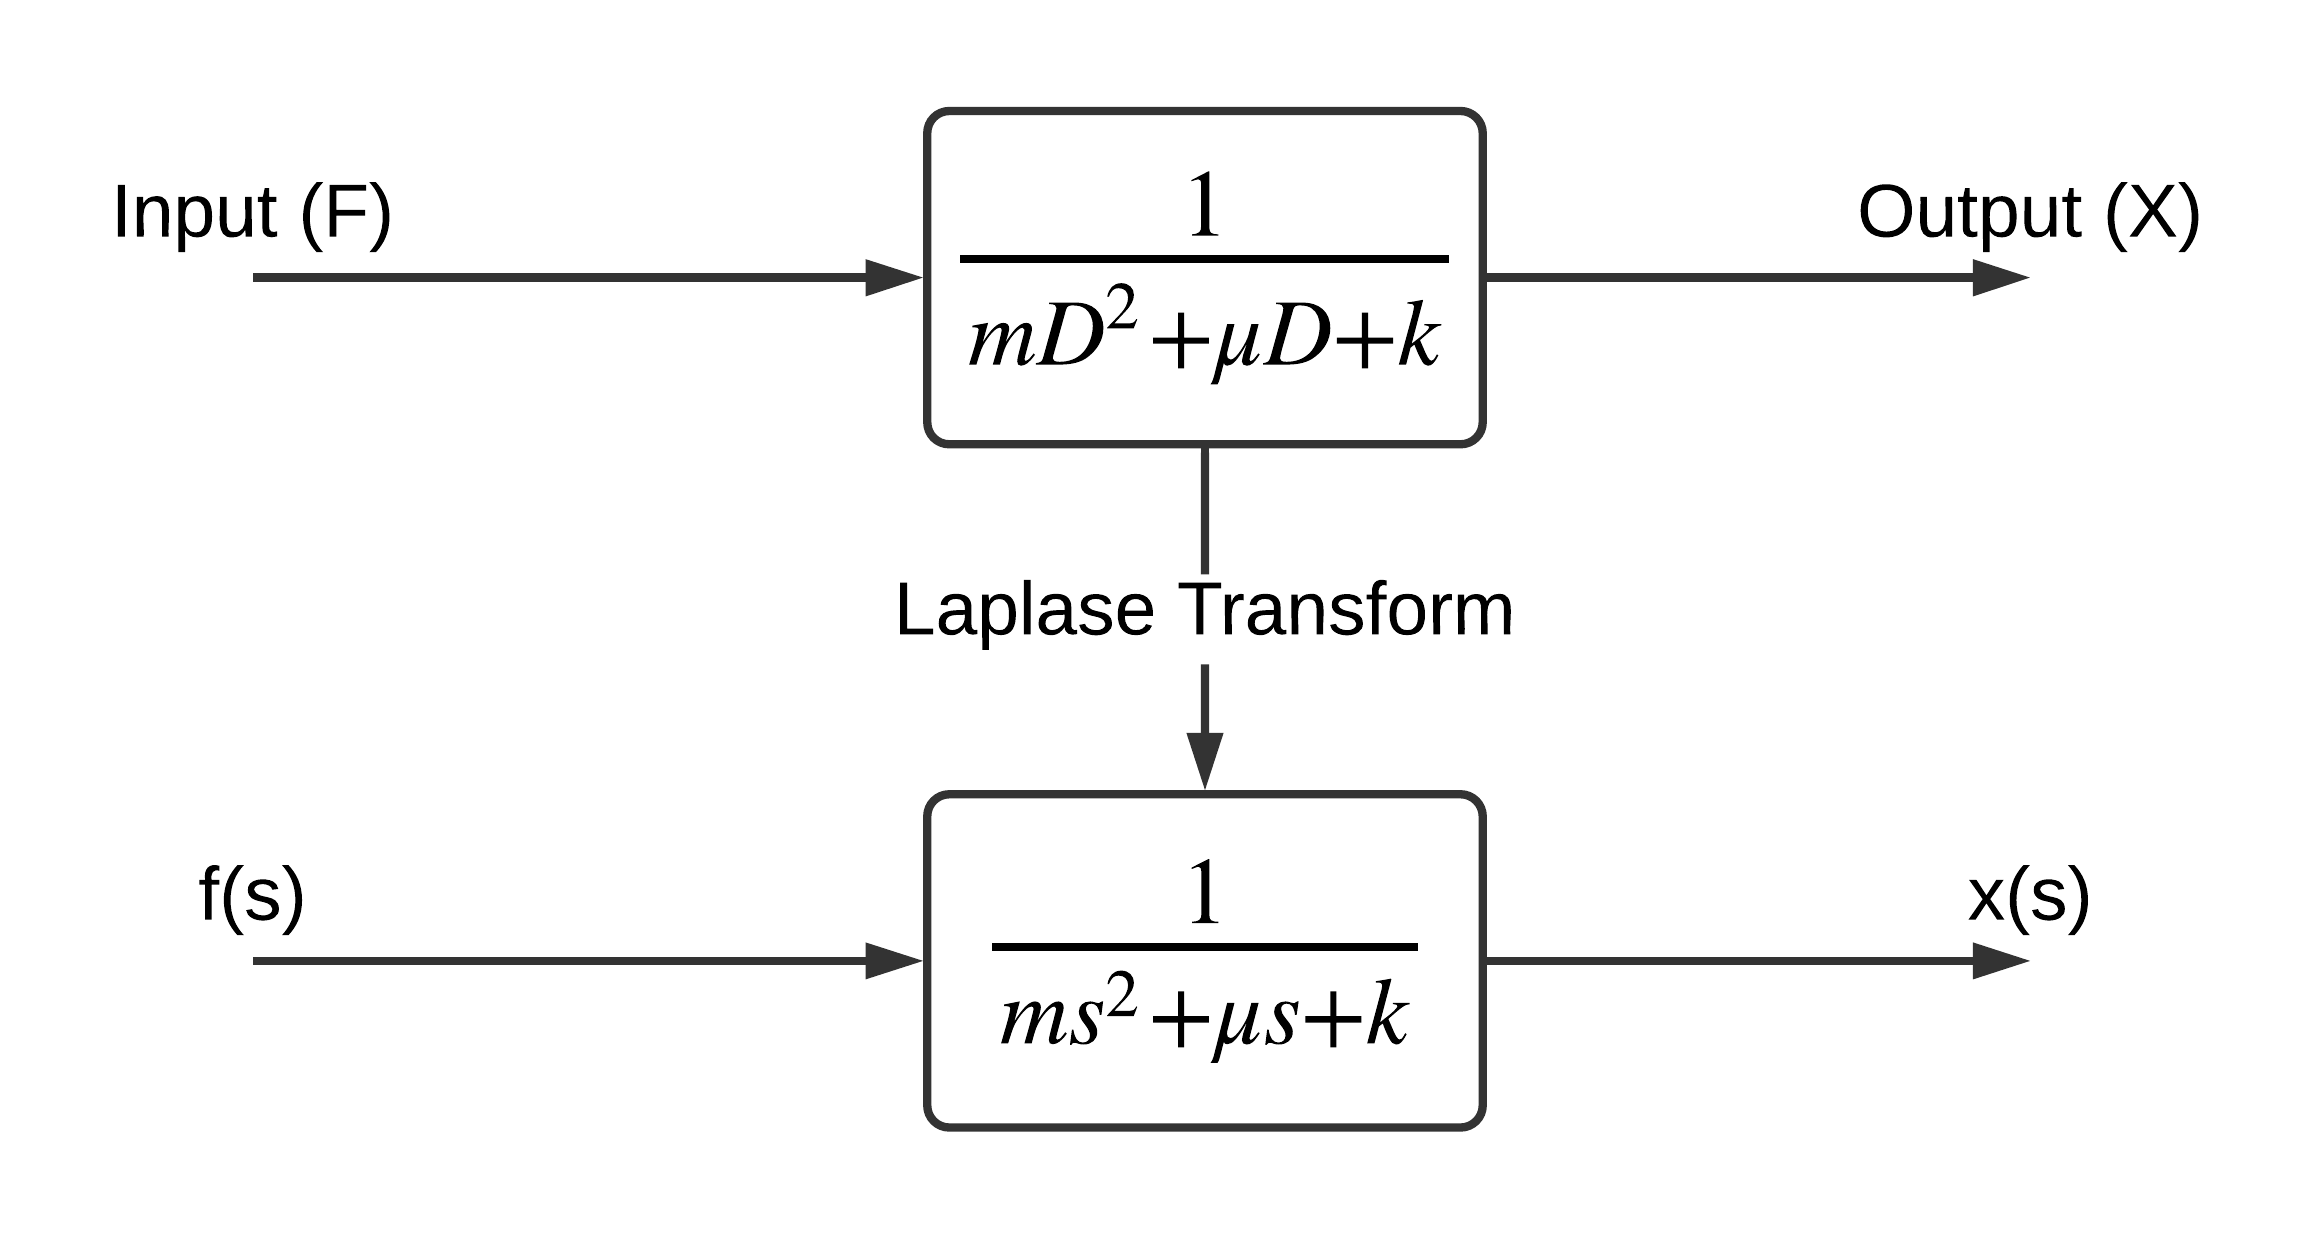
\includegraphics[width=0.65\textwidth]{lec1/Better Block Diagram}
		\caption[Spring problem: block diagram]{Since D is an operator (can't have a value),  the transfer function is obtained by the Laplace transform of the first relation.}
		\labfig{dynamicsSystemBlockDiagram}
\end{figure}
\todo{Switch cases to match Laplase}
\leavevmode\\[-1.3cm]

\begin{description}
	\item[Transfer function] ratio between Laplace transform of the output and Laplace transform of the input, assuming zero initial conditions.
\end{description}
 \leavevmode\\[-5em]

\section{Control Systems}
\labsec{sec1.2}
A control system is an interconnection of components forming a system configuration that will provide a desired system response.
\\[-2em]

\subsection[Open-loop control system]{Open-loop control system (without feedback):}
\begin{figure}[hb]
		\raggedleft
		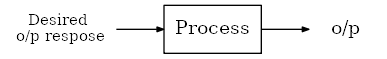
\includegraphics[width=0.41\textwidth]{lec1/Open-loop control system}
		\caption[Open-loop: block diagram]{Its output does not track the input, and it is more affected by noise.}
		\labfig{openLoopBlockDiagram}
\end{figure}
 \leavevmode\\[-4em]

\subsection[Closed-loop control system]{Closed-loop feedback control system (with feedback):}

\begin{figure}[hb]
		\raggedleft
		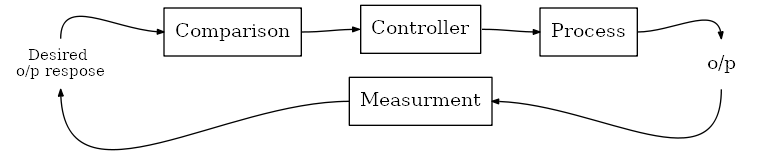
\includegraphics[width=0.8\textwidth]{lec1/Closed-loop control system}
		\caption[Closed-loop: block diagram]{Closed loop control can improve accuracy, also the actuating signal is a function of the output.}
		\labfig{closedLoopBlockDiagram}
\end{figure}

\section{Mathematical Model}
Any linear continuous system can be represented either by a linear algebraic equation or an ordinary differential equation such as:\\[-4mm]

%https://tex.stackexchange.com/questions/195774/how-to-right-align-any-line-or-word-in-a-paragraph-in-any-documentclass
\hspace*{\fill} $(mD^2 + \mu D + k)\ x(t) = y(t)$\\[-4mm]

Solving the differential equation using Laplace transform assuming zero initial conditions made it possible to get the transfer function.

\todo{Add copyrights to lec.}
\section{Block Diagram Reduction}

\begin{margintable}[-0.5cm]
\caption[Canonical form of feedback control system]{Terminology}
\labtab{canonicalTable}
\centering
\tiny
 	\begin{tabular}{|c c l|}
	        \hline
	        \multicolumn{3}{c}{}\\[-1em]
	        R &: & reference input / desired output response.\\
	        E &: & actuating / error signal.\\
	        G &: & control element and controlled system.\\
	        C &: & controlled variable / actual output.\\
	        H &: & feedback / backward transfer element.\\
	        B &: & primary feedback.\\
	        s &: & summation point.\\
	        t &: & takeoff point.\\
	        \multicolumn{3}{c}{}\\[-1em]
	        \hline
	    \end{tabular}
\end{margintable}

\begin{marginfigure}[-0.5cm]
		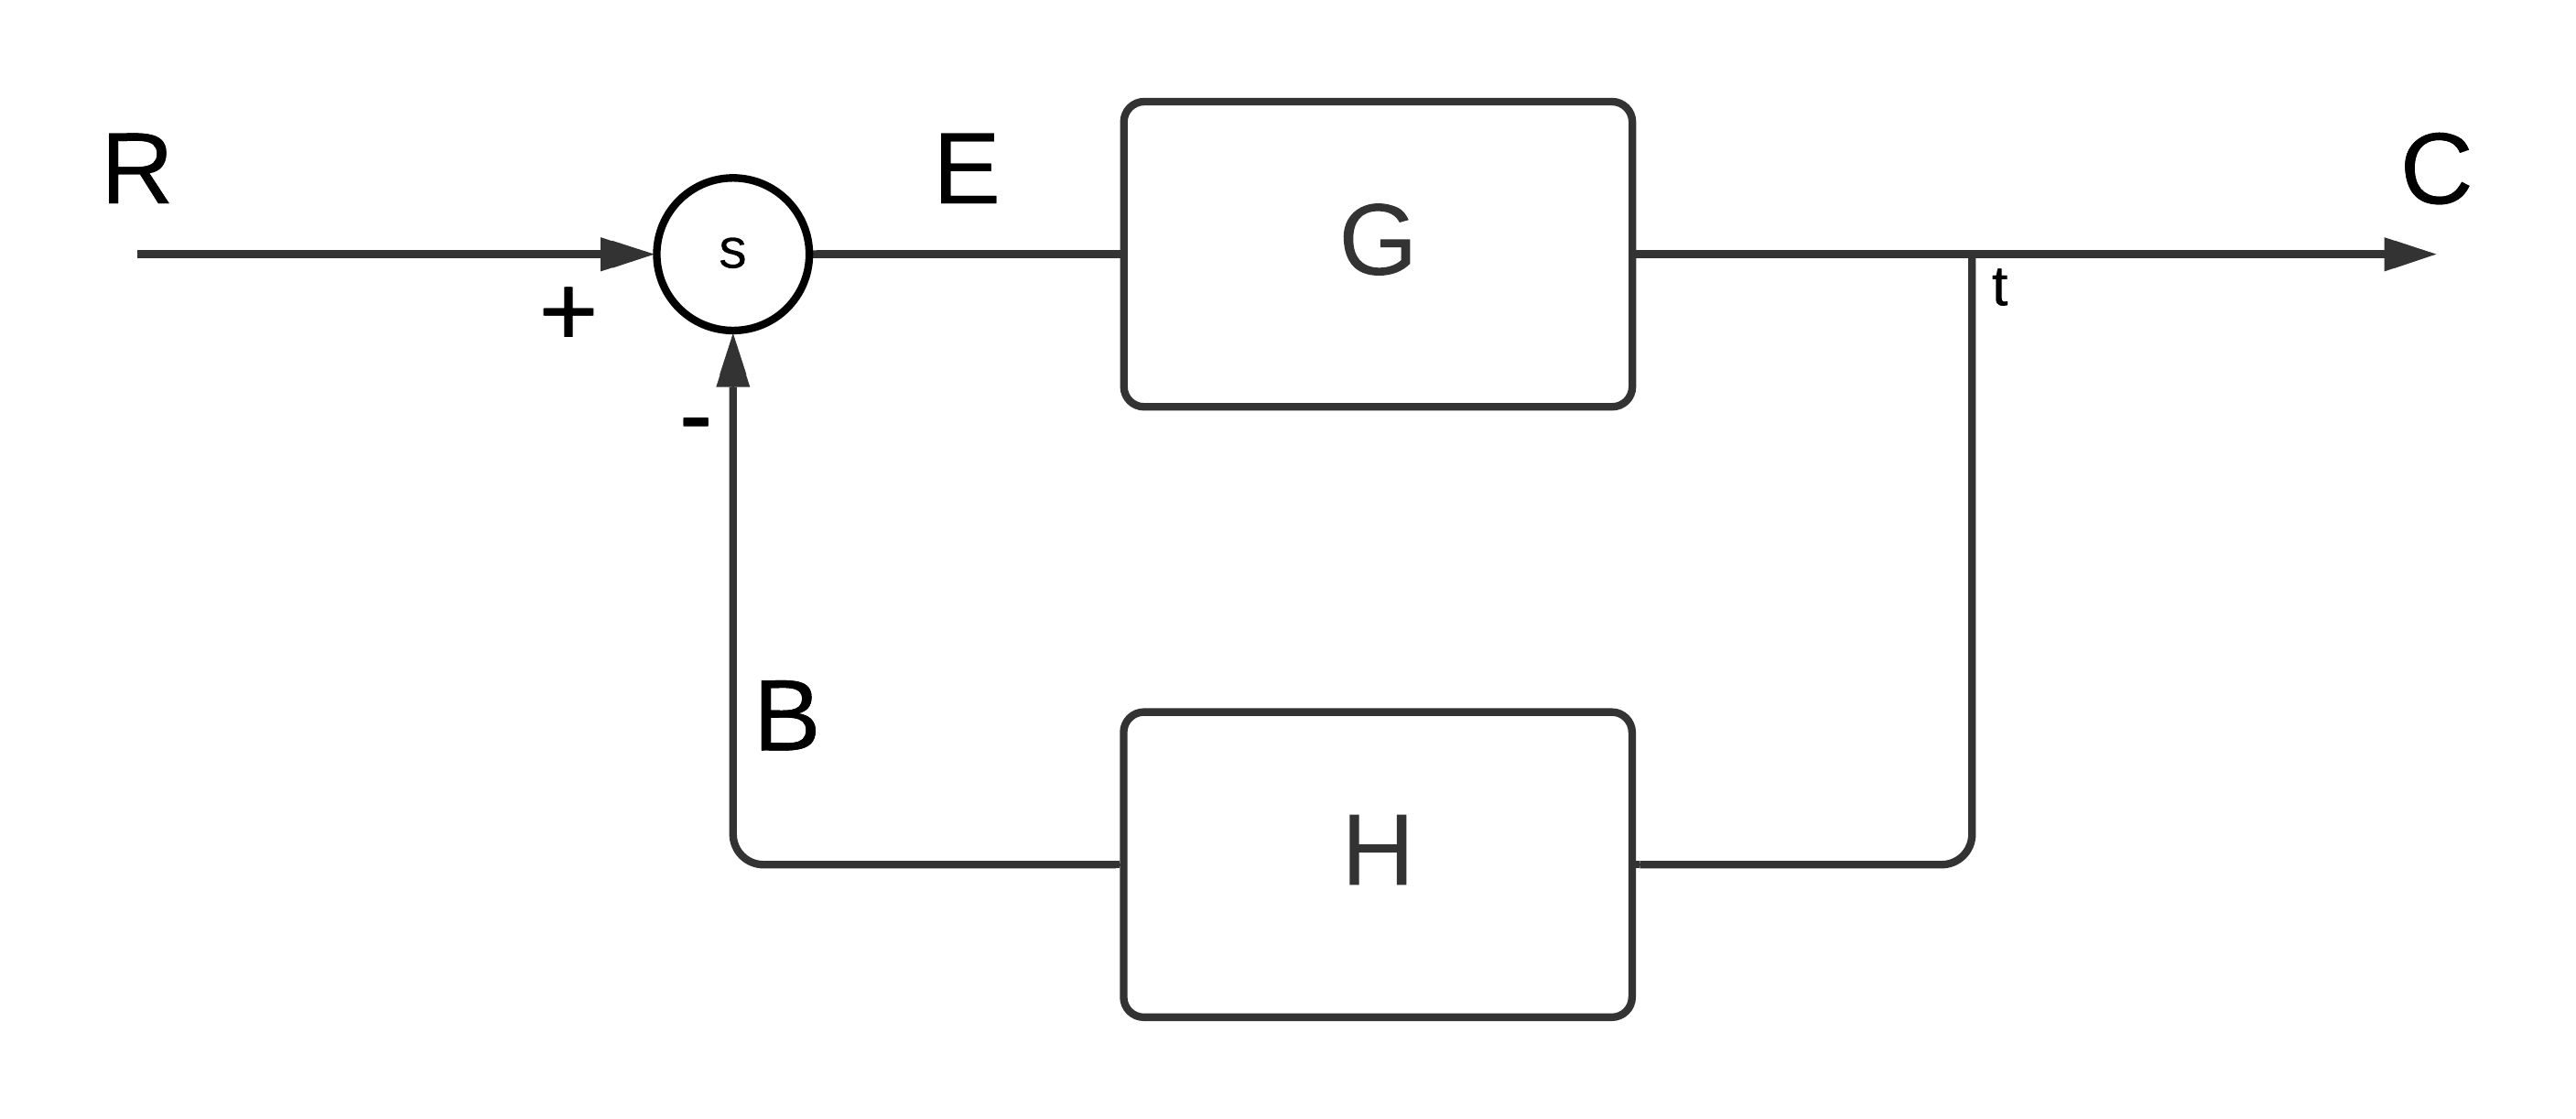
\includegraphics{lec1/Canonical Block Diagram}
		\caption[Canonical form: block diagram]{Canonical feedback loop.}
		\labfig{canonicalBlockDiagram}
\end{marginfigure}
\todo{negative feedback}
A Block Diagram is a shorthand pictorial representation of the cause-and-effect relationship of a system.
Control systems require the arithmetic manipulation in order to obtain the overall transfer function and
this is the start point for the analysis of the system.\\

\begin{tabular}{r p{0.1cm} c}
Cascade connection & : &\\
					&&  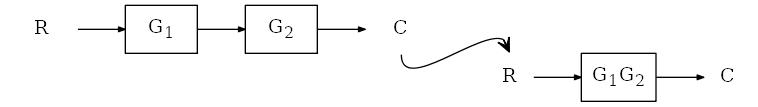
\includegraphics[width=0.6\textwidth]{lec1/Series Both}\\
Parallel connection & : &\\
					&&  \tiny\ \ \ 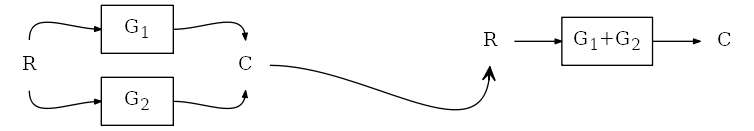
\includegraphics[width=0.6\textwidth]{lec1/Parallel Both}\\
					&& \\
Summation point & : &\\
					&&  \multicolumn{1}{p{6.5cm}}{\scriptsize a small circle, with plus or minus sign associated with the inputs,
					and the output is the algebraic sum of the inputs.}\\
Take-off point & : &\\
					&&   \multicolumn{1}{p{6.5cm}}{\scriptsize a takeoff (or pickoff) point is used in order 
					to have the same signal input to more than one block.}\\
\end{tabular}

\subsection[Overall transfer function]{Overall transfer function (feedback loop elimination):}
Applying reduction techniques mentioned above, we can obtain the overall transfer function of \reffig{canonicalBlockDiagram} 

\todo{Give more space between each pair}

\begin{tabular}{r c l r}
	\multicolumn{2}{c}{$@\ s:$} & $E = R - B$ & \note{summation point}\\
			&$\because  $& $B = CH$ & \note{block}\\
			&$\therefore$& $E = R - CH$ &\\
			&$\because  $& $C = GE$ & \note{block}\\
			&$\therefore$& $C = G(R-CH)$ &\\
			&& $C + CGH = GR$ & \\
			&& $C(1+GH) = GR$ & \\
			&&&
			\fbox{
			    \parbox{2.25cm}{
			    $\dfrac{C}{R} = \dfrac{G}{(1+GH)}$
		    		}
			}\\[-2mm]
\end{tabular}

\begin{marginfigure}[-1cm]
		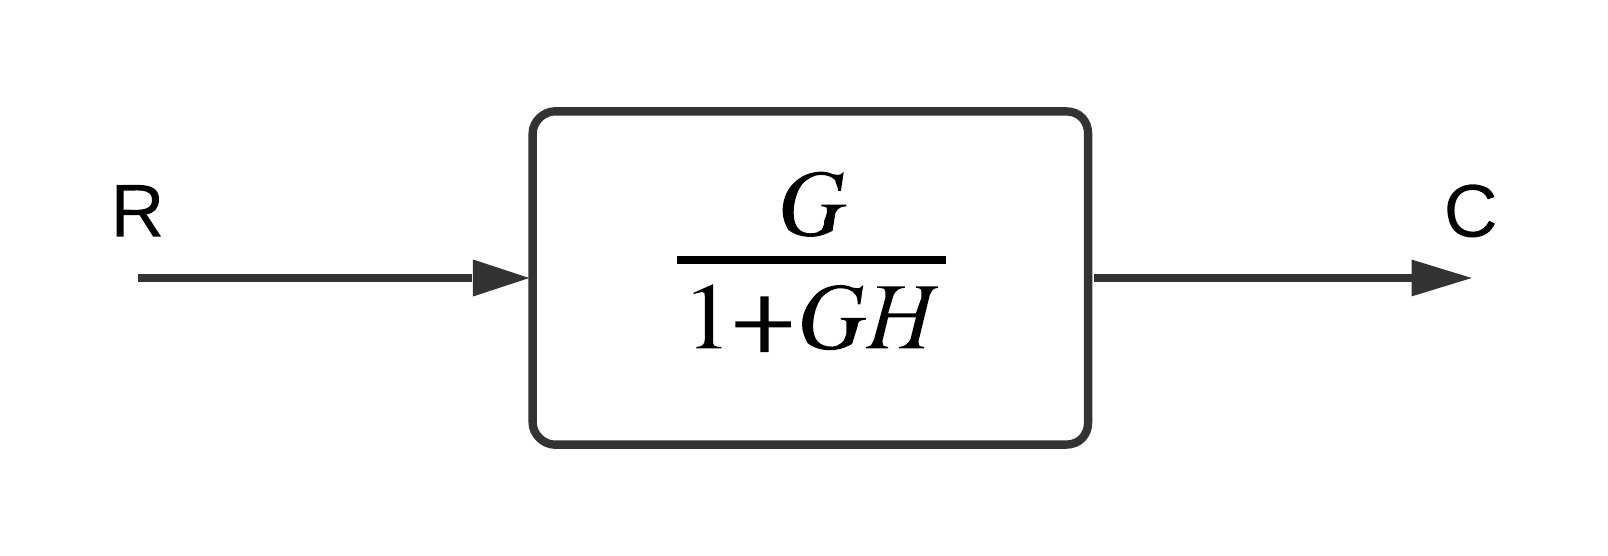
\includegraphics{lec1/Reduction Example Formula}
		\caption[Overall transfer function: block diagram]{Feedback loop equivalent}
		\labfig{OverallTransferBlockDiagram}
\end{marginfigure}

$End\ ?$
\todo{Missed super position in multi i/p and postponed the mathematical models}